\documentclass[paper=letter, fontsize=11pt]{scrartcl} % Letter paper and 11pt font size
\usepackage{lmodern}
\usepackage[T1]{fontenc}
\usepackage[spanish]{babel}
\usepackage[utf8]{inputenc}
\usepackage{amssymb}
\usepackage{fullpage}
\usepackage{latexsym}
\usepackage{enumerate}
\usepackage{enumitem}
\usepackage{graphicx}
\PassOptionsToPackage{hyphens}{url}\usepackage{hyperref}
\title{Topología: Tarea \#10}
\newtheorem{lemma}{Lema}

%\usepackage{fourier} % Use the Adobe Utopia font for the document - comment this line to return to the LaTeX default
\usepackage{amsmath,amsfonts,amsthm} % Math packages

\usepackage{lipsum}
\makeatletter
\renewcommand\lips@dolipsum{%
  \ifnum\value{lips@count}<\lips@max\relax
    \addtocounter{lips@count}{1}%
    \csname lipsum@\romannumeral\c@lips@count\endcsname
    \lips@dolipsum
  \fi
}
\makeatother % Used for inserting dummy 'Lorem ipsum' text into the template

\usepackage{sectsty} % Allows customizing section commands
\allsectionsfont{\centering \normalfont\scshape} % Make all sections centered, the default font and small caps

\usepackage{fancyhdr} % Custom headers and footers
\pagestyle{fancyplain} % Makes all pages in the document conform to the custom headers and footers
\fancyhead{} % No page header - if you want one, create it in the same way as the footers below
\fancyfoot[L]{} % Empty left footer
\fancyfoot[C]{} % Empty center footer
\fancyfoot[R]{\thepage} % Page numbering for right footer
\renewcommand{\headrulewidth}{0pt} % Remove header underlines
\renewcommand{\footrulewidth}{0pt} % Remove footer underlines
\setlength{\headheight}{13.6pt} % Customize the height of the header

\numberwithin{equation}{section} % Number equations within sections (i.e. 1.1, 1.2, 2.1, 2.2 instead of 1, 2, 3, 4)
\numberwithin{figure}{section} % Number figures within sections (i.e. 1.1, 1.2, 2.1, 2.2 instead of 1, 2, 3, 4)
\numberwithin{table}{section} % Number tables within sections (i.e. 1.1, 1.2, 2.1, 2.2 instead of 1, 2, 3, 4)

% \setlength\parindent{0pt} % Removes all indentation from paragraphs - comment this line for an assignment with lots of text

%----------------------------------------------------------------------------------------
%	TITLE SECTION
%----------------------------------------------------------------------------------------

\newcommand{\horrule}[1]{\rule{\linewidth}{#1}} % Create horizontal rule command with 1 argument of height

\newcommand{\prob}[1]{\mathbb{P}(#1)}
\newcommand{\pr}[1]{\mathbb{P}_{#1}}

\title{	
\normalfont \normalsize 
\textsc{universidad de los andes, departamento de matemáticas} \\ [25pt] % Your university, school and/or department name(s)
\horrule{0.5pt} \\[0.4cm] % Thin top horizontal rule
\huge Probabilidad (Honores): Parcial 2 \\ % The assignment title
\horrule{2pt} \\[0.5cm] % Thick bottom horizontal rule
}

\author{Jonathan Andrés Niño Cortés} % Your name

\date{\normalsize\today} % Today's date or a custom date
\begin{document}
\maketitle

\section{Ejercicio 1}

\begin{enumerate}[label = \Alph*)]
\item \begin{enumerate}[label = \arabic*)]
\item Sea $ \mu_1 $ una distribución en $ \mathbb{R} $. Calcule el parámetro $ c \in \mathbb{R} $ que falta.
\begin{equation}
\mu_1(dx)=c\frac{1}{x}\mathbb{I}\{x>2\}dx \nonumber
\end{equation}

\item Sea $ \mu_2 $ una distribución en $ \mathbb{R} $. Calcule el parametro $ c \in \mathbb{R} $ que falta.
\begin{equation}
\mu_2(dx)=5\frac{1}{x^c}\mathbb{I}\{x>1\}dx \nonumber
\end{equation}

\item Sea $ \mu_3 $ una distribución en $ \mathbb{R} $. Calcule el parametro $ c \in \mathbb{R} $ que falta.
\begin{equation}
\mu_3(dx)=5\frac{\ln(x)}{x^c}\mathbb{I}\{x>1\}dx \nonumber
\end{equation}
\end{enumerate}

\begin{proof}
Para que una distribución $  \mu $ este bien definida, es necesario que la integral
\begin{equation}
\int_{-\infty}^{\infty}\mu(dx)=1 \nonumber
\end{equation}

\begin{enumerate}[label = \arabic*)]
\item 
\begin{eqnarray}
\int_{-\infty}^{\infty}\mu_1(dx) &=& \int_{-\infty}^{\infty} c\frac{1}{x}\mathbb{I}\{x>2\}dx \nonumber
\\ &=& \int_{2}^{\infty} c\frac{1}{x}dx \nonumber
\\ &=& \lim_{t \to \infty} \int_{2}^{t} c\frac{1}{x}dx \nonumber
\\ &=& \lim_{t \to \infty} c\ln(x)\bigg |_{2}^t \nonumber
\\ &=& \lim_{t \to \infty} c\ln(t)-c\ln(2) \nonumber
\\ &=& c\infty \nonumber
\end{eqnarray}

Luego, no hay ningún valor de $ c $ tal que esta integral de 1.
\item Por lo que vimos anteriormente $ c\leq1 $ no va a funcionar, pues la integral impropia no va a converger. Entonces asumimos que $ c > 1 $.
\begin{eqnarray}
\int_{-\infty}^{\infty}\mu_2(dx) &=& \int_{-\infty}^{\infty} 5\frac{1}{x^c}\mathbb{I}\{x>1\}dx \nonumber
\\ &=& \int_{1}^{\infty} 5\frac{1}{x^c}dx \nonumber
\\ &=& \lim_{t \to \infty} \int_{1}^{t} 5\frac{1}{x^c}dx \nonumber
\\ &=& \lim_{t \to \infty} 5\frac{1}{(1-c)x^{c-1}}\bigg |_{1}^t \nonumber
\\ &=& \lim_{t \to \infty} 5\big(\frac{1}{c-1}-\frac{1}{(c-1)t^{c-1}}\big) \nonumber
\\ &=& \frac{5}{c-1} \nonumber
\end{eqnarray}

Por lo tanto, $ c = 6 $ es el parámetro que le falta a la distribución probabilística.

\item Por lo que vimos anteriormente $ c\leq1 $ no va a funcionar, pues la integral impropia no va a converger. Entonces asumimos que $ c > 1 $.
\begin{eqnarray}
\int_{-\infty}^{\infty}\mu_3(dx) &=& \int_{-\infty}^{\infty} 5\frac{\ln(x)}{x^c}\mathbb{I}\{x>1\}dx \nonumber
\\ &=& \int_{1}^{\infty} 5\frac{\ln(x)}{x^c}dx \nonumber
\\ &=& \lim_{t \to \infty} \int_{1}^{t} 5\frac{\ln(x)}{x^c}dx \nonumber
\\ &=& \lim_{t \to \infty} 5\frac{\ln(x)}{(1-c)x^{c-1}}\bigg|_{1}^t - \int_{1}^{t} 5\frac{1}{(1-c)x^{c}} \nonumber \text{ (Integración por partes)}
\\ &=& \lim_{t \to \infty} 5\frac{\ln(x)}{(1-c)x^{c-1}}\bigg|_{1}^t - 5\frac{1}{(1-c)^2x^{c-1}} \bigg|_{1}^t \nonumber
\\ &=& \lim_{t \to \infty} 5\frac{\ln(t)}{(1-c)t^{c-1}}-5\frac{\ln(1)}{(1-c)1^{c-1}} - 5\frac{1}{(1-c)^2t^{c-1}}+5\frac{1}{(1-c)^21^{c-1}} \nonumber
\\ &=& \lim_{t \to \infty} \frac{5\ln(t)}{(1-c)t^{c-1}}- \frac{5}{(1-c)^2t^{c-1}}+\frac{5}{(1-c)^2} \nonumber
\\ &=& \frac{5}{(1-c)^2} +\lim_{t \to \infty} \frac{5\ln(t)}{(1-c)t^{c-1}}  \nonumber
\\ &=& \frac{5}{(1-c)^2} +\lim_{t \to \infty} \frac{5\frac{1}{t}}{-(1-c)^2t^{c-2}} \text{ (L'Hopital)} \nonumber
\\ &=& \frac{5}{(1-c)^2} +\lim_{t \to \infty} \frac{5}{-(1-c)^2t^{c-1}} \nonumber
\\ &=& \frac{5}{(1-c)^2} \nonumber
\end{eqnarray}


Entonces el parametro para completar la distribución es $ c = \sqrt{5}+1 $.
\end{enumerate}

\end{proof}
\item Considere una familia enumerable de variables aleatorias $ (X_i)_{i \in \mathbb{N}} $ con $ X_i \sim \mathcal{U}_{[0,1]}  $.
\begin{enumerate}[label = \arabic*)]
	\setcounter{enumii}{3}
\item Calcule y dibuje la densidad de $ X_1 + X_2 $.
\begin{proof}
Para calcular la densidad de la suma de variables independientes debemos calcular la convolución de las densidades de las variables que se van a sumar.

La función de densidad de una variable $ X_i $ es $ f_i=\mathbb{I}\{0 \leq x \leq 1\}  $.

Entonces la función de densidad $ g $ de $ X_1 + X_2 $ es
\begin{eqnarray}
g(x)= \int_{\mathbb{R}} f_1(t)f_2(x-t)dt \nonumber
\\g(x)= \int_{\mathbb{R}} \mathbb{I}\{0 \leq t \leq 1\}\mathbb{I}\{0 \leq x-t \leq 1\}dt \nonumber
\end{eqnarray}

Entonces debemos considerar dos casos diferentes. Si $ x < 1 $ o si $ x \geq 1$. En el primer caso tenemos que $ \mathbb{I}\{0 \leq t \leq 1\}\mathbb{I}\{0 \leq x-t \leq 1\} = 1 $ si y solo si $ 0<t<x $. Luego

\begin{equation}
g(x)= \int_{\mathbb{R}} \mathbb{I}\{0 \leq t \leq 1\}\mathbb{I}\{0 \leq x-t \leq 1\}dt = \int_0^x dt = t\bigg|_0^x=x \nonumber
\end{equation}

En el segundo caso entonces tenemos que $ \mathbb{I}\{0 \leq x \leq 1\}(t)\mathbb{I}\{0 \leq x \leq 1\}(x-t) = 1 $ si y solo si $ x-1<t<1 $. Luego
\begin{equation}
g(x)= \int_{\mathbb{R}} \mathbb{I}\{0 \leq t \leq 1\}\mathbb{I}\{0 \leq x-t \leq 1\}dt = \int_x-1^1 dt = t\bigg|_{x-1}^1=2-x \nonumber
\end{equation}

Entonces $ g(x) = x\mathbb{I}\{0\leq x \leq 1\} +(2-x)\mathbb{I}\{1\leq x \leq 2\} $

La gráfica de esta función es

$$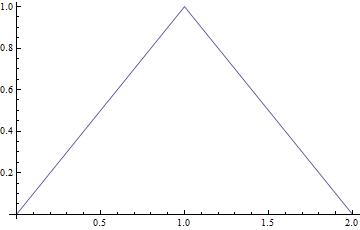
\includegraphics{Grafica1}$$
\end{proof}

\item Calcule y dibuje la densidad de $ X_1 + X_2+X_3 $.
\begin{proof}
Como ya calculamos la función de densidad de $ X_1+X_2 $ la función de densidad de $ X_1+X_2+X_3 $ la podemos calcular como la convolución de $ g $ y $ f_3 $. Defina esta convolución por $ h $.

\begin{eqnarray}
h(x)&=& \int_{\mathbb{R}} g(t)f_3(x-t)dt \nonumber
\\h(x)&=& \int_{\mathbb{R}} [t\mathbb{I}\{0\leq t \leq 1\} +(2-t)\mathbb{I}\{1\leq t \leq 2\}]\mathbb{I}\{0 \leq x-t \leq 1\}dt \nonumber
\\h(x)&=& \int_{\mathbb{R}} t\mathbb{I}\{0\leq t \leq 1\}\mathbb{I}\{0 \leq x-t \leq 1\}dt + \int_{\mathbb{R}} (2-t)\mathbb{I}\{1\leq t \leq 2\}\mathbb{I}\{0 \leq x-t \leq 1\}dt \nonumber
\end{eqnarray}

De nuevo cada integral la debemos calcular por casos. Si $ x < 1 $ entonces como el caso anterior tenemos que la primera integral es diferente de 0 si $ 0<t<x $, mientras que la segunda integral siempre es 0. Luego

\begin{equation}
h(x) = \int_{0}^x tdx = \frac{t^2}{2}\bigg|_0^x=\frac{x^2}{2}\nonumber
\end{equation}

Para el caso en que $ 1 \leq x < 2 $ entonces la primera integral es diferente de 0 si $ x-1<t<1 $ y la segunda integral es diferente de 0 si $ 1 < t <x $.

Entonces 

\begin{eqnarray}
h(x) &=& \int_{x-1}^1 tdt + \int_{1}^x (2-t)dt = \frac{t^2}{2}\bigg|_{x-1}^1 + (2t-\frac{t^2}{2})\bigg|_{1}^x = \frac{1}{2}-\frac{(x-1)^2}{2}+2x-\frac{x^2}{2}-(2-\frac{1}{2}) \nonumber
\\h(x)&=& -x^2+3x-\frac{3}{2}  \nonumber
\end{eqnarray}

Finalmente si $ x \leq 2 $ la primera integral siempre es 0 mientras que la segunda es diferente de 0 cuando $ x-1<t<2$. Entonces

\begin{equation}
h(x)=\int_{x-1}^{2} (2-t)dt = (2t-\frac{t^2}{2})\bigg|_{x-1}^2 = (4-2)-\bigg(2(x-1)-\frac{(x-1)^2}{2}\bigg) = \frac{x^2}{2} -3x+\frac{9}{2}\nonumber
\end{equation}

Y entonces la función de distribución $ \displaystyle \mathbb{I}\{0\leq x \leq 1\}\frac{t^2}{2}+\mathbb{I}\{1\leq x \leq 2\}(-x^2+3x-\frac{3}{2})+\mathbb{I}\{2\leq x \leq 3\}(\frac{x^2}{2}-3x+\frac{9}{2}) $.

La gráfica de esta función es

$$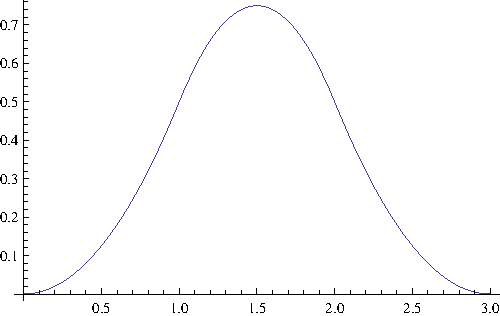
\includegraphics{Grafica02}$$
\end{proof}

\item Calcule y dibuje la densidad de $ X_1 + X_2 + X_3 + X_4 $.

\begin{proof}
De nuevo tenemos que calcular la densidad $ j(x) $ como la convolución de $ h $ y $ f_4 $.

\begin{eqnarray}
j(x) &=& \int_{\mathbb{R}} h(x)f_4(x-t)dt \nonumber
\\ &=& \int_{\mathbb{R}} \bigg(\mathbb{I}\{0\leq t \leq 1\}\frac{t^2}{2}+\mathbb{I}\{1\leq t \leq 2\}(-t^2+3t-\frac{3}{2})+\mathbb{I}\{2\leq t \leq 3\}(\frac{t^2}{2}-3t+\frac{9}{2})\bigg)\mathbb{I}\{0\leq x-t \leq 1\}dt \nonumber
\\&=& \int_{\mathbb{R}} \mathbb{I}\{0\leq t \leq 1\}\mathbb{I}\{0\leq x-t \leq 1\}\frac{t^2}{2}dt + \int_{\mathbb{R}} \mathbb{I}\{1\leq t \leq 2\}\mathbb{I}\{0\leq x-t \leq 1\}(-t^2+3t-\frac{3}{2})dt \nonumber
\\& & + \int_{\mathbb{R}} \mathbb{I}\{2\leq t \leq 3\}\mathbb{I}\{0\leq x-t \leq 1\}(\frac{t^2}{2}-3t+\frac{9}{2})dt  \nonumber 
\end{eqnarray}

Entonces de nuevo tenemos que considerar cuatro casos diferentes. Si $ x < 1 $ entonces la única integral que no es cero es la primera y justo no es cero cuando $ 0<t<x $.

 \begin{equation}
 j(x)=\int_{0}^x \frac{t^2}{2} dt = \frac{t^3}{6}\bigg|_0^x = \frac{x^3}{6}. \nonumber
 \end{equation}

El segundo caso es cuando $ 1 \leq x \leq  2 $. Entonces la primera integral es diferente de 0 cuando $ x-1 < t < 1 $ y la segunda integral es diferente de 0 cuando $ 1 < t < x $. 

\begin{eqnarray}
j(x)&=&\int_{x-1}^1 \frac{t^2}{2}dt + \int_1^x \bigg(-t^2+3t-\frac{3}{2}\bigg)dt \nonumber
\\ &=& \frac{t^3}{6}\bigg|_{x-1}^1+\bigg(-\frac{t^3}{3}+\frac{3t^2}{2}-\frac{3t}{2}\bigg)\bigg|_{1}^x\nonumber
\\&=& \frac{1}{6}-\frac{(x-1)^3}{6}+\bigg(-\frac{x^3}{3}+\frac{3x^2}{2}-\frac{3x}{2} \bigg) - \bigg( -\frac{1}{3}+\frac{3}{2}-\frac{3}{2} \bigg) \nonumber
\\&=& \frac{1}{6}-\frac{x^3}{6}+\frac{x^2}{2}-\frac{x}{2}+\frac{1}{6}-\frac{x^3}{3}+\frac{3x^2}{2}-\frac{3x}{2}+\frac{1}{3} \nonumber
\\&=& -\frac{x^3}{2}+2x^2-2x+\frac{2}{3} \nonumber
\end{eqnarray}

El tercer caso es cuando $ 2\leq x \leq 3 $ y en este caso la segunda integral es no cero cuando $ x-1<t<2 $ y la tercera integral es no cero cuando $ 2<t<x $.

\begin{eqnarray}
j(x) &=& \int_{x-1}^2 \bigg(-t^2+3t-\frac{3}{2}\bigg)dt + \int_{2}^x \bigg(\frac{t^2}{2}-3t+\frac{9}{2}\bigg) \nonumber
\\&=& \bigg(-\frac{t^3}{3}+\frac{3t^2}{2}-\frac{3t}{2}\bigg)\bigg|_{x-1}^2+ \bigg(\frac{t^3}{6}-\frac{3t^2}{2}+\frac{9t}{2} \bigg)\bigg|_2^x \nonumber
\\&=& \bigg(-\frac{8}{3}+{6}-3\bigg)-\bigg(-\frac{(x-1)^3}{3}+\frac{3(x-1)^2}{2}-\frac{3(x-1)}{2}\bigg)+\bigg(\frac{x^3}{6}-\frac{3x^2}{2}+\frac{9x}{2} \bigg)-\bigg(\frac{8}{6}-6+9 \bigg) \nonumber
\\&=& -\frac{8}{3}+3+\frac{x^3}{3}-x^2+x-\frac{1}{3}-\frac{3x^2}{2}+3x-\frac{3}{2}+\frac{3x}{2}-\frac{3}{2}+\frac{x^3}{6}-\frac{3x^2}{2}+\frac{9x}{2}-\frac{4}{3}-3 \nonumber
\\&=& \frac{x^3}{2}-4x^2+10x-\frac{22}{3} \nonumber
\end{eqnarray}

Finalmente tenemos el caso cuando $ x > 3 $. En este caso la única integral que sobrevive es la ultima y no es cero cuando $ x-1 $ a $ 3 $.

\begin{eqnarray}
j(x) &=& \int_{x-1}^3 \bigg(\frac{t^2}{2}-3t+\frac{9}{2}\bigg)dt \nonumber
\\&=& \bigg(\frac{t^3}{6}-\frac{3t^2}{2}+\frac{9t}{2}\bigg) \bigg|_{x-1}^3 \nonumber
\\&=& \bigg(\frac{9}{2}-\frac{27}{2}+\frac{27}{2}\bigg)-\bigg(\frac{(x-1)^3}{6}-\frac{3(x-1)^2}{2}+\frac{9(x-1)}{2}\bigg)  \nonumber
\\&=& \frac{9}{2}-\frac{x^3}{6}+\frac{x^2}{2}-\frac{x}{2}+\frac{1}{6}+\frac{3x^2}{2}-3x+\frac{3}{2}-\frac{9x}{2}+\frac{9}{2}
\nonumber
\\ &=& -\frac{x^3}{6}+2x^2-8x+\frac{32}{3} \nonumber \end{eqnarray}

Finalmente obtenemos que $ j(x) =\mathbb{I}\{0\leq x\leq 1\}\frac{x^3}{6} + \mathbb{I}\{1\leq x\leq 2\}(-\frac{x^3}{2}+2x^2-2x+\frac{2}{3})+\mathbb{I}\{2\leq x\leq 3\}(\frac{x^3}{2}-4x^2+10x-\frac{22}{3})+ \mathbb{I}\{3\leq x\leq 4\}( -\frac{x^3}{6}+2x^2-8x+\frac{32}{3}) $

La gráfica de esta función es

$$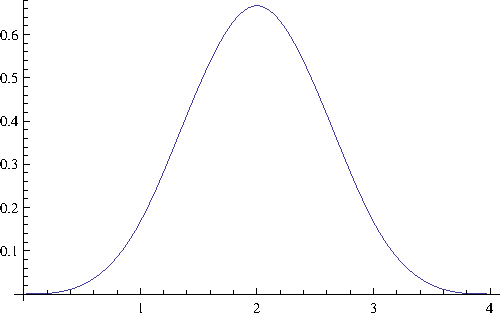
\includegraphics{Grafica3}$$

Finalmente mostramos una gráfica que incluye las tres funciones juntas

$$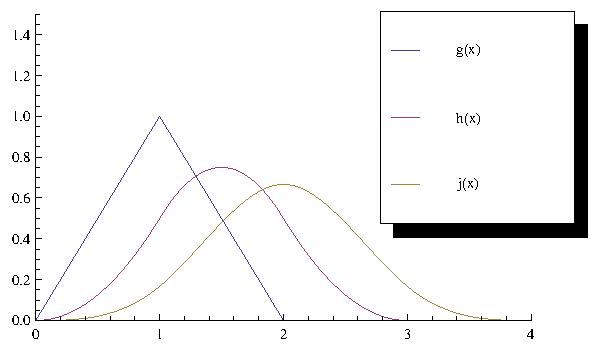
\includegraphics{Grafica4}$$
\end{proof}
\item Qué sospecha sobre la densidad de $ \sum_{i=1}^n X_i $? Coleccione toda la información que usted sospecha.

\begin{proof}
Denote por $ g_n $ la función de masa de $ \sum_{i=1}^n X_i $. Una de las cosas que podemos demostrar es que las funciones $ g_n $ son continuas y alcanzan su maximo en $ \frac{n}{2} $. También podemos observar que son simétricas con respecto a la recta $ x = \frac{n}{2} $, es decir que $ g_n(x)=g(n-x) $. Una de las cosas que sospecho es que los valores que toma esta función en punto enteros debe aproximarse a los valores que tomaría la distribución binomial $ \mathcal{B}_{n,\frac{1}{2}} $
\end{proof}

\end{enumerate}
\item Demuestre por cálculo directo para variables aleatorias $ \bot(X,Y) $ las siguientes implicaciones:
\begin{enumerate}[label = \arabic*)]
	\setcounter{enumii}{7}
	\item $ X \sim \mathcal{P}_\lambda $, $ Y \sim \mathcal{P}_{\lambda'} $ entonces $ X + Y \sim \mathcal{P}_{\lambda+\lambda'} $.
	
	\begin{proof}
	Para nuestras variables discretas independientes $ X $ y $ Y $ la función de masa $ f  $ de $ X+ Y $ esta dada por
	
	\begin{equation}
	f(x) = \sum_{t=0}^x f_1(t)f_2(x-t) \nonumber
	\end{equation}
	
	donde $ f_1 $ y $ f_2 $ son las funciones de masa de $ X $ y $ Y $ respectivamente.
	
	Ahora las funciones de masa de la distribución de Poission son $ \displaystyle f_1(x) = \frac{e^{-\lambda}\lambda^x}{x!}  $ y  $ \displaystyle f_2(x) = \frac{e^{-\lambda'}(\lambda')^x}{x!}$.
	
	Luego la función de masa de $ X+Y $ esta dada por
	
	\begin{eqnarray}
	f(x) &=& \sum_{t=0}^x f_1(t)f_2(x-t) \nonumber
	\\ &=& \sum_{t=0}^x \frac{e^{-\lambda}\lambda^t}{t!}\frac{e^{-\lambda'}(\lambda')^{x-t}}{(x-t)!} \nonumber
	\\&=& e^{-(\lambda+\lambda')}\sum_{t=0}^x\frac{\lambda^t(\lambda')^{x-t}}{t!(x-t)!} \nonumber
	\end{eqnarray}
	
	Recordemos que el coeficiente binomial esta definido como $ \displaystyle \binom{x}{k} = \frac{x!}{k!(x-k)!} $. Luego tenemos que $ \displaystyle \frac{1}{k!(x-k)!} =  \frac{1}{x!}\binom{x}{k} $.
	
	Por lo tanto nuestra expresión resultante es
	
	\begin{eqnarray}
	f(x) &=& e^{-(\lambda+\lambda')}\sum_{t=0}^x\frac{\lambda^t(\lambda')^{x-t}}{t!(x-t)!} \nonumber 
	\\&=& e^{-(\lambda+\lambda')}\sum_{t=0}^x \frac{1}{x!}\binom{x}{t}\lambda^t(\lambda')^{x-t} \nonumber \\&=&\frac{e^{{-(\lambda+\lambda')}}}{x!}\sum_{t=0}^x \binom{x}{t}\lambda^t(\lambda')^{x-t} \nonumber
	\end{eqnarray}
	
	Pero vemos que la sumatoria que queda es precisamente la fórmula binomial de Newton para el polinomio $ (\lambda+\lambda')^x $, luego la fórmula final es
	
	\begin{equation}
	f(x) = \frac{e^{-(\lambda+\lambda')}(\lambda+\lambda')^x}{x!} \nonumber
	\end{equation}
	
	
	Que coincide precisamente con la función de masa asociada a $ \mathcal{P}_{\lambda+\lambda'} $.
	\end{proof}
	
	\item $ X \sim \mathcal{B}_{n_1,p} $, $ Y \sim \mathcal{B}_{n_2,p} $ entonces $ X+Y \sim \mathcal{B}_{n_1+n_2,p} $.
	
	\begin{proof}
	En este caso las funciones de masa asociadas a $ X $ y $ Y $ son respectivamente $ \displaystyle f_1(x)=\binom{n_1}{x}p^x(1-p)^{n_1-x}  $ y $ \displaystyle f_2(x)=\binom{n_2}{x}p^x(1-p)^{n_2-x}  $.
	Entonces la función de masa de $ X+ Y $ esta dada por
	
	\begin{eqnarray}
	f(x) &=& \sum_{t=0}^x f_1(t)f_2(x-t) \nonumber
	\\ &=& \sum_{t=0}^x \binom{n_1}{t}p^t(1-p)^{n_1-t}\binom{n_2}{x-t}p^{x-t}(1-p)^{n_2-(x-t)}  \nonumber
	\\&=& \sum_{t=0}^x \binom{n_1}{t}\binom{n_2}{x-t}p^{t+x-t}(1-p)^{n_1-t+n_2-(x-t)}  \nonumber
	\\&=& \sum_{t=0}^x \binom{n_1}{t}\binom{n_2}{x-t}p^{x}(1-p)^{n_1+n_2-x}  \nonumber
	\\&=& p^{x}(1-p)^{n_1+n_2-x}  \sum_{t=0}^x \binom{n_1}{t}\binom{n_2}{x-t} \nonumber
	\end{eqnarray}
	
	Ahora concentrandonos en los coeficientes binomiales una de sus definiciones es que $ \binom{n}{k} $ es el coeficiente que acompaña al $ k $-ésimo término del polinomio $ (x+1)^n$.
	
	Entonces si tomamos $ (x+1)^{n_1+n_2}=(x+1)^{n_1}(x+1)^{n_2} $ y por definición de la multiplicación de polinomios, el $ x $-ésimo término estaria dado por $ \sum_{t=0}^{x}a_{t}b_{x-t} $, es decir, $ \displaystyle \binom{n_1+n_2}{x}= \sum_{t=0} \binom{n_1}{t}\binom{n_2}{x-t} $.
	
	Por lo tanto, llegamos a la expresió final
	
	\begin{equation}
	f(x) = p^{x}(1-p)^{n_1+n_2-x}  \sum_{t=0}^x \binom{n_1}{t}\binom{n_2}{x-t} = \binom{n_1+n_2}{x} p^{x}(1-p)^{n_1+n_2-x}\nonumber	
	\end{equation}
	
	que es la función de masa asociada a $ \mathcal{B}_{n_1+n_2,p} $.
	\end{proof}
	
	\item $ X \sim N_{m_1,\sigma_1^2} $, $ Y \sim N_{m_2,\sigma_2^2} $ entonces $ X+Y \sim N_{m_1+,m_2,\sigma_1^2+\sigma_2^2} $.
	\begin{proof}
	En este caso debemos utilizar las funciones de densidad de $ X $ y $ Y $ que son respectivamente $ \displaystyle f_1(x) = \frac{1}{\sigma_1\sqrt{2\pi}}e^{-\frac{(x-m_1)^2}{2\sigma_1^2}} $ y $ \displaystyle  f_2(x)= \frac{1}{\sigma_2\sqrt{2\pi}}e^{-\frac{(x-m_2)^2}{2\sigma_2^2}}  $.
	
	Entonces la función de densidad asociada $ X+Y $ esta dada por
	
	\begin{eqnarray}
	f(x) &=& \int_{\mathbb{R}} \frac{1}{\sigma_1\sqrt{2\pi}}e^{-\frac{(t-m_1)^2}{2\sigma_1^2}}\frac{1}{\sigma_2\sqrt{2\pi}}e^{-\frac{(x-t-m_2)^2}{2\sigma_2^2}}dt \nonumber
	\\&=&  \frac{1}{\sigma_1\sigma_22\pi}\int_{\mathbb{R}}e^{-\frac{(t-m_1)^2}{2\sigma_1^2}-\frac{(x-t-m_2)^2}{2\sigma_2^2}} \nonumber dt
	\\&=&  \frac{1}{\sigma_1\sigma_22\pi}\int_{\mathbb{R}}e^{-\frac{(t-m_1)^2}{2\sigma_1^2}-\frac{(x-t-m_2)^2}{2\sigma_2^2}} \nonumber dt
	\end{eqnarray}
	
	Para simplificar los cálculos utilizamos la sustitución $ z = t-m_1 $.
	
	\begin{eqnarray}
	f(x) &=&
	\frac{1}{\sigma_1\sigma_22\pi}\int_{\mathbb{R}}e^{-\frac{z^2}{2\sigma_1^2}-\frac{(x-m_1-m_2-z)^2}{2\sigma_2^2}} \nonumber dz
	\end{eqnarray}
	
	Y tome $ a = x-m_1-m_2 $, pues todos estos son constantes en la integral.
	
	\begin{eqnarray}
	f(x) &=& 	\frac{1}{\sigma_1\sigma_22\pi}\int_{\mathbb{R}}e^{-\frac{z^2}{2\sigma_1^2}-\frac{(a-z)^2}{2\sigma_2^2}} \nonumber dz
	\\&=& \frac{1}{\sigma_1\sigma_22\pi}\int_{\mathbb{R}}e^{-\frac{\sigma_2^2z^2+\sigma_1^2(a-z)^2}{2\sigma_1^2\sigma_2^2}} \nonumber dz
	\\&=& \frac{1}{\sigma_1\sigma_22\pi}\int_{\mathbb{R}}e^{-\frac{\sigma_2^2z^2+\sigma_1^2(z^2-2az+a^2)}{2\sigma_1^2\sigma_2^2}} \nonumber dz
	\\&=& \frac{1}{\sigma_1\sigma_22\pi}\int_{\mathbb{R}}e^{-\frac{(\sigma_1^2+\sigma_2^2)z^2-2\sigma_1^2az+\sigma_1^2a^2}{2\sigma_1^2\sigma_2^2}} \nonumber dz
	\end{eqnarray}
	
	Ahora podemos completar cuadrados al polinomio $ (\sigma_1^2+\sigma_2^2)z^2-2\sigma_1^2az+\sigma_1^2a^2 $
	
%	\begin{eqnarray}
%	& &(\sigma_1^2+\sigma_2^2)t^2-2t(\sigma_1^2(x-m_2)+\sigma_2^2m_1)+\sigma_1^2(x-m_2)^2+\sigma_2^2m_1^2 \nonumber
%	\\&=&(\sigma_1^2+\sigma_2^2)t^2-2t\sqrt{\sigma_1^2+\sigma_2^2}\frac{\sigma_1^2(x-m_2)+\sigma_2^2m_1}{\sqrt{\sigma_1^2+\sigma_2^2}}+\frac{(\sigma_1^2(x-m_2)+\sigma_2^2m_1)^2}{\sigma_1^2+\sigma_2^2}+ \nonumber
%	\\& & \sigma_1^2(x-m_2)^2+\sigma_2^2m_1^2-\frac{(\sigma_1^2(x-m_2)+\sigma_2^2m_1)^2}{\sigma_1^2+\sigma_2^2} \nonumber
%	\\&=&\Big(\sqrt{\sigma_1^2+\sigma_2^2}t-\frac{\sigma_1^2(x-m_2)+\sigma_2^2m_1}{\sqrt{\sigma_2^2+\sigma_2}}\Big)^2 + (\sigma_1^2(x-m_2)^2+\sigma_2^2m_1^2)(1-\frac{\sigma_1^2(x-m_2)^2+\sigma_2^2m_1^2}{\sigma_1^2+\sigma_2^2}) \nonumber
%	\\&=&\frac{((\sigma_1^2+\sigma_2^2)t-\sigma_1^2(x-m_2)-\sigma_2^2m_1)^2}{\sigma_1^2+\sigma_2^2} + (\sigma_1^2(x-m_2)^2+\sigma_2^2m_1^2)(\frac{\sigma_1^2+\sigma_2^2-\sigma_1^2(x-m_2)^2-\sigma_2^2m_1^2}{\sigma_1^2+\sigma_2^2}) \nonumber
%	\end{eqnarray}

\begin{eqnarray}
&&(\sigma_1^2+\sigma_2^2)z^2-2\sigma_1^2az+\sigma_1^2a^2 \nonumber
\\&=& (\sigma_1^2+\sigma_2^2)z^2-2\sqrt{\sigma_1^2+\sigma_2^2}\frac{\sigma_1^2a}{\sqrt{\sigma_1^2+\sigma_2^2}}z  +\frac{\sigma_1^4a^2}{\sigma_1^2+\sigma_2^2}+\sigma_1^2a^2-\frac{\sigma_1^4a^2}{\sigma_1^2+\sigma_2^2}\nonumber
\\&=& (\sqrt{\sigma_1^2+\sigma_2^2}z-\frac{\sigma_1^2a}{\sqrt{\sigma_1^2+\sigma_2^2}})^2 +\sigma_1^2a^2-\frac{\sigma_1^4a^2}{\sigma_1^2+\sigma_2^2}\nonumber
\end{eqnarray}

Entonces nuestra integral resultante es

\begin{eqnarray}
f(z)&=& \frac{1}{\sigma_1\sigma_22\pi}\int_{\mathbb{R}}e^{\frac{(\sqrt{\sigma_1^2+\sigma_2^2}z-\frac{\sigma_1^2a}{\sqrt{\sigma_1^2+\sigma_2^2}})^2 +\sigma_1^2a^2-\frac{\sigma_1^4a^2}{\sigma_1^2+\sigma_2^2}}{2\sigma_1^2\sigma_2^2}} \nonumber dz
\\&=&\frac{1}{\sigma_1\sigma_22\pi}\int_{\mathbb{R}}e^{(\frac{\sqrt{\sigma_1^2+\sigma_2^2}}{\sqrt{2}\sigma_1\sigma_2}z-\frac{\sigma_1^2a}{\sqrt{2}\sigma_1\sigma_2\sqrt{\sigma_1^2+\sigma_2^2}})^2 +\frac{a^2}{2\sigma_2^2}-\frac{\sigma_1^2a^2}{2\sigma_2^2(\sigma_1^2+\sigma_2^2)}} \nonumber dz
\end{eqnarray}

Por último realize la sustitución $ \displaystyle w = \frac{\sqrt{\sigma_1^2+\sigma_2^2}}{\sqrt{2}\sigma_1\sigma_2}z-\frac{\sigma_1a}{\sqrt{2}\sigma_2\sqrt{\sigma_1^2+\sigma_2^2}} $ y tome $ \displaystyle b = \frac{a^2}{2\sigma_2^2}-\frac{\sigma_1^2a^2}{2\sigma_2^2(\sigma_1^2+\sigma_2^2)} =  \frac{a^2}{2\sigma_2^2}(1-\frac{\sigma_1^2}{\sigma_1^2+\sigma_2^2}) =\frac{a^2}{2\sigma_2^2}\frac{\sigma_1^2+\sigma_2^2-\sigma_1^2}{\sigma_1^2+\sigma_2^2} = \frac{a^2}{2(\sigma_1^2+\sigma_2^2)}.$

Entonces la integral resultante es

\begin{eqnarray}
f(x)&=&\frac{1}{\sqrt{2}\pi\sqrt{\sigma_1^2+\sigma_2^2}}\int_{\mathbb{R}}e^{-w^2-b} \nonumber dw
\\&=& \frac{e^{-b}}{\sqrt{2}\pi\sqrt{\sigma_1^2+\sigma_2^2}}\int_{\mathbb{R}}e^{-w^2} \nonumber dw
\end{eqnarray}
El valor de esta integral es igual a $ \sqrt{\pi} $. Luego obtenemos la expresión.

\begin{eqnarray}
f(x)&=&\frac{e^{-b}}{\sqrt{2}\pi\sqrt{\sigma_1^2+\sigma_2^2}}\sqrt{\pi} \nonumber
\\&=&\frac{e^{-b}}{\sqrt{2\pi}\sqrt{\sigma_1^2+\sigma_2^2}}\nonumber
\\&=&\frac{1}{\sqrt{2\pi}\sqrt{\sigma_1^2+\sigma_2^2}}e^{- \frac{a^2}{2(\sigma_1^2+\sigma_2^2)}} \nonumber
\\&=&\frac{1}{\sqrt{2\pi}\sqrt{\sigma_1^2+\sigma_2^2}}e^{- \frac{(x-m_1-m_2)^2}{2(\sigma_1^2+\sigma_2^2)}} \nonumber
\end{eqnarray}

Que es precisamente la función de densidad asociada a $ N_{m_1+m_2,\sigma_1^2+\sigma_2^2} $
\end{proof}
\end{enumerate}
\end{enumerate}

\section{Ejercicio 2}

En un típico texto alemán, la letra  e  es la más frecuente con un 12.5\% de todas las letras. Un sofware repasa un texto desconocido  puramente aleatoriamente  y reconoce con la certeza de 99\% la letra  e  correctamente. Con la probabilidad 0.1\% reconoce una  e  erroneamente.

\begin{enumerate}[label = \arabic*.]
\item Qué tan grande es la probabilidad que el sofware indique la letra  e  en un paso?

\begin{proof}
Vamos a modelar el espacio de estados como $ \Omega:=\{E,\neg E\}\times \{D_e, \neg D_e\} $, donde $ E $ denote leer una e, y $ \neg E $ su negación, mientras que $ D_e $ denota detectar una e, y $ \neg D_e $ denota su negación.

Entonces vamos a definir los estados $ A = \{(E,D_e),(E,\neg D_e)\} $ y $ B=\{(E,D_e),(\neg E,D_e)\} $. donde $ A $ es leer una e y $ B $ es detectar una e.

El enunciado nos indica que $ \mathbb{P}(A)=0.125 $ por lo que $ \mathbb{P}(A^C)=1-\mathbb{P}(A)=0.875 $.

Además nos indica que $ \mathbb{P}(B|A) = 0.99 $ y que $ \mathbb{P}(B|A^C)=0.001 $.

Entonces por la fórmula de probabilidad total, como $ A $ y $ A^C $ forman una partición del espacio $ \Omega $, tenemos que $ \displaystyle \mathbb{P}(B)=\prob{A}\mathbb{P}(B|A)+\prob{A^C}\prob{B|A^C} = 0.125*0.99+0.875*0.001 = 0.1252375 = \frac{10019}{80000}
 $.
\end{proof}

\item Qué tan grande es la probabilidad que es efectivamente la letra  e  cuando detecta una  e ?

\begin{proof}
Esta probabilidad la podemos calcular usando la fórmula de Bayes. Tenemos que $ \displaystyle \prob{A|B} = \frac{\prob{B|A}\prob{A}}{\prob{B}} = \frac{0.99*0.125}{0.1252375} = \frac{0.12375}{0.1252375}= \frac{9900}{10019}$
\end{proof}
\end{enumerate}

\section{Ejercicio 3: Sin memoria implica la distribución exponencial o geométrica}

\begin{enumerate}[label = \arabic*)]
\item Demuestre que para toda las variables aleatorias con valores $ [0, \infty) $ cuya distribución $ \mathbb{P}_X $ es absolutamente continua con respecto a la medida de Lebesgue con una densidad estrictamente positiva y que satisface

\begin{equation}
\forall t,s > 0,\qquad 0 <\prob{X>t+s|X>t}=\prob{X>s}<1 \nonumber
\end{equation}
existe un $ \lambda > 0 $ tal que $ \mathbb{P}_X = \text{EXP}(\lambda) $.

\begin{proof}
En primer lugar vamos a desarrollar un poco más la expresión de la no memoria. Por Bayes tenemos que

\begin{equation}
\prob{X>s}=\prob{(X>t+s|X>t)}=\frac{\prob{X>t|X>t+s}\prob{X>t+s}}{\prob{X>t}} \nonumber
\end{equation}

Pero ahora tenemos que si $ X>t+s $ entonces $ X>t $, luego $ \prob{X>t|X>t+s} = 1 $.

Luego tenemos que

\begin{eqnarray}
\prob{X>s}&=&\frac{\prob{X>t+s}}{\prob{X>t}} \nonumber
\\\prob{X>t}\prob{X>s}&=&\prob{X>t+s} \nonumber
\end{eqnarray}

Ahora recordemos que la función $ F(x) $ asociada a la distribución esta definida como $ F(x)= \prob{X\leq x} $. Luego $ \prob{X>x}= 1-\prob{X \leq x} = 1 - F(x) $.

Entonces podemos escribir la expresión anterior como
\begin{equation}
(1-F(t))(1-F(s))=1-F(s+t) \nonumber
\end{equation}

Ahora si tomamos logaritmos tenemos que
\begin{eqnarray}
\ln((1-F(t)(1-F(s))&=&\ln(1-F(s+t)) \nonumber
\\\ln(1-F(t)+\ln(1-F(s))&=&\ln(1-F(s+t)) \nonumber
\end{eqnarray}
Entonces vemos que la función $ h(x)=\ln(1-F(x)) $ es un automorfismo continuo de $ \mathbb{R} $ que preserva la suma.

Entonces podemos demostrar que $ h(x)= \lambda x $ para algún $ \lambda \in \mathbb{R} $. Tome $ \lambda = h(1) $. Primero si $ x \in \mathbb{N} $ podemos demostrar por inducción que $ h(x)=xh(1) $. Ahora si tomamos $ x \in \mathbb{Z} $ con $ x <= 0 $ tenemos que $ h(0)=h(1-1)=h(1)+h(-1)=0 $ por lo que $ h(-1)=-h(1) $, luego por inducción podemos demostrar que $ h(x)=xh(1) $.

Ahora para $ x \in \mathbb{Q} $ consideremos sin pérdida de generalidad el caso cuando $ x = \frac{1}{n} $ para $ n \in \mathbb{N}\backslash\{0\} $. Entonces tenemos que $ f(1)=\underbrace{f(\frac{1}{n})+\cdots+f(\frac{1}{n})}_{n\text{ veces}} $. Luego por inducción podemos probar que $ f(1)=nf(\frac{1}{n}) $ por lo que $ f(\frac{1}{n})= \frac{1}{n}f(1) $. Ya teniendo $ \frac{1}{n} $ podemos calcular $ f(\frac{m}{n}) $ para cualquier $ m \in \mathbb{Z} $ y probar como para los enteros que $ f(\frac{m}{n})=m f(\frac{1}{n})= \frac{m}{n}f(1) $.

Finalmente podemos demostrar que $ h(x)=h(1)x $ para cualquier $ x \in X $ porque ya demostramos que $ h\upharpoonright_{\mathbb{Q}}(x)=h(1)x $. Por topología sabemos que $ \mathbb{Q} $ es denso en $ \mathbb{R} $ y además tenemos un teorema que si $ f $ y $ g $ son dos funciones continuas de $ X $, $ D $ es denso en $ X $ y las funciones son tales que $ f(x)=g(x) $ para cualquier $ x \in D $ entonces $ f(x)=g(x) $ para cualquier $ x \in X $. Este teorema nos permite concluir que $ h(x)= h(1)x= \lambda x $.

Entonces volviendo a la expresión anterior tenemos que $ h(x)=\ln(1-F(x))=\lambda x $. Luego tomando exponencial a ambos lados tenemos que $ 1-F(x)= e^{\lambda x} $ por lo que $ F(x)=1-e^{\lambda x} $. Finalmente sabemos que la función de densidad se calcula como $ f(x) = F'(x) $, entonces $ f(x)= -\lambda e^{\lambda x} $. Como una de las hipotesis es que la distribución es absolutamente continua $ f(x) $ debe ser siempre positivo por lo que $ \lambda<0 $. Por lo que podemos escribir $ f(x)= \lambda'e^{-\lambda'x} $ con $ \lambda' = -\lambda > 0 $, que es precisamente la función de densidad asociada a la distribución exponencial con parámetro $ \lambda' $
\end{proof}
\item Demuestre que para todas las variables aleatorias $ X $ con valores en $ \mathbb{N} $ cuya distribución $ \mathbb{P}_X $ satisface

\begin{equation}
\prob{X>n+m|X>m}=\prob{X>m}<1 \qquad \forall n,m \in \mathbb{N}\backslash \{0\} \nonumber
\end{equation}

\begin{proof}
Por el mismo argumento que en el punto anterior llegamos a que

\begin{equation}
\prob{X>n}\prob{X>m}=\prob{X>n+m} \nonumber
\end{equation}

Ahora podemos escribir $ \prob{X>x}=1-\prob{X\leq x} 1-\sum_{i=1}^x \prob{X=i} $, por lo que la expresión queda como

\begin{equation}
(1-\sum_{i=1}^n \prob{X=i})(1-\sum_{i=1}^m \prob{X=i})=(1-\sum_{i=1}^{n+m} \prob{X=i})
\end{equation}

Ahora vamos a demostrar por inducción fuerte que
 \begin{equation}
 (1-\sum_{i=1}^x \prob{X=i}) = q^x
 \end{equation}
 
 para algún $ q \in \mathbb{R} $.

Para el caso base tenemos que $ 1-\sum_{i=1}^1 \prob{X=i} = 1-\prob{X=1} $. Entonces si tomamos $ q = 1-\prob{X=1} $ vemos que se cumple la condición.

Ahora por la hipótesis de la no memoria tenemos que para cualquier $ x>1  $, $\displaystyle 1-\sum_{i=1}^x \prob{X = i} = (1-\sum_{i=1}^n \prob{X=i})(1-\sum_{i=1}^m \prob{X=i}) $. para algunos $ n,m \in \mathbb{N} \backslash \{0\} $. Entonces por la hipotesis de inducción tenemos que  $ \displaystyle 1-\sum_{i=1}^x \prob{X = i} = q^nq^m=q^{n+m}= q^x $.

Esto nos permite calcular $ \prob{X = x} $ pues 
\begin{equation}
\prob{X=x}= 1-\sum_{i=1}^{x-1}\prob{X=i}-(1-\sum_{i=1}^{x} \prob{X=i}) = q^{x-1}-q^{x} = q^{x-1}(1-q). \nonumber
\end{equation}

Finalmente tenemos que $ \sum_{i=1}^\infty \prob{X=i} = (1-q)\sum_{i=1}^\infty q^{x-1} $ debe converger y debe ser mayor que 0. Por lo tanto, como esta es la serie geométrica tenemos que $ 0 \leq q < 1 $. Por ultimo si tomamos $ p = 1- q $ tendriamos que $ \prob{X=x} = p(1-p)^{x-1} $ con $ 0<p\leq 1 $ y por lo tanto tiene asociada la distribución geométrica con parámetro $ p $.
\end{proof}
\end{enumerate}

\section{Ejercicio 4}

\begin{enumerate}[label = \arabic*)]
\item Sea $ X = (X_1,X_2):\Omega \to \{0,1,2\}^2 $ un vector aleatorio con marginales
\begin{eqnarray}
\mathbb{P}_{X_1}&=&\alpha_0\delta_0+\alpha_1\delta_1+\alpha_2\delta_2 \nonumber
\\\mathbb{P}_{X_2}&=&\beta_0\delta_0+\beta_1\delta_1+\beta_2\delta_2 \nonumber
\end{eqnarray}

Construya el sistema lineal de todas las ecuaciones y reduzcalo lo máximo posible con el algoritmo de Gauss. Cuántos grados de libertad existen para estas leyes de $ \mathbb{P}_X $ en el espacio producto $ \{0,1,2\}^2 $?
\begin{proof}
Denotamos $ \pr{ij}:=\prob{X_1=i \cap X_2 = j} $. De estas ecuaciones marginales deducimos el siguiente sistema de ecuaciones.

\begin{eqnarray}
\alpha_0 &=&\pr{00}+\pr{01}+\pr{02} \nonumber
\\\alpha_1 &=& \pr{10}+\pr{11}+\pr{12} \nonumber
\\\alpha_2 &=& \pr{20}+\pr{21}+\pr{22} \nonumber
\\\beta_0 &=& \pr{00}+\pr{10}+\pr{20} \nonumber
\\\beta_1 &=& \pr{01}+\pr{11}+\pr{21} \nonumber
\\\beta_2 &=& \pr{02}+\pr{12}+\pr{22} \nonumber
\end{eqnarray}

Entonces la matriz asociada a este sistema es
\begin{equation}
\begin{pmatrix}
1 & 1 & 1 & 0 & 0 & 0 & 0 & 0 & 0
\\0 & 0 & 0 & 1 & 1 & 1 & 0 & 0 & 0
\\0 & 0 & 0 & 0 & 0 & 0 & 1 & 1 & 1
\\1 & 0 & 0 & 1 & 0 & 0 & 1 & 0 & 0
\\0 & 1 & 0 & 0 & 1 & 0 & 0 & 1 & 0
\\0 & 0 & 1 & 0 & 0 & 1 & 0 & 0 & 1
\end{pmatrix} \nonumber
\end{equation}

Y la matriz escalonada reducida resultante del algoritmo de Gauss (calculada mediante Wolfram Mathematica) es

\begin{equation}
\begin{pmatrix}
 1 & 0 & 0 & 0 & -1 & -1 & 0 & -1 & -1 \\
 0 & 1 & 0 & 0 & 1 & 0 & 0 & 1 & 0 \\
 0 & 0 & 1 & 0 & 0 & 1 & 0 & 0 & 1 \\
 0 & 0 & 0 & 1 & 1 & 1 & 0 & 0 & 0 \\
 0 & 0 & 0 & 0 & 0 & 0 & 1 & 1 & 1 \\
 0 & 0 & 0 & 0 & 0 & 0 & 0 & 0 & 0
\end{pmatrix} \nonumber
\end{equation}
Por lo que vemos que los grados de libertad para estas leyes son 5.
\end{proof}

\item Sea $ X = (X_1,X_2,X_3):\Omega \to \{0,1\}^3 $ un vector aleatorio con marginales
\begin{eqnarray}
\mathbb{P}_{X_1}&=&\alpha_0\delta_0+\alpha_1\delta_1, \nonumber
\\\mathbb{P}_{X_2}&=&\beta_0\delta_0+\beta_1\delta_1, \nonumber
\\\mathbb{P}_{X_3}&=&\gamma_0\delta_0+\gamma_1\delta_1, \nonumber
\end{eqnarray}

Construya el sistema lineal de todas las ecuaciones y reduzcalo lo máximo posible con el algoritmo de Gauss. Cuántos grados de libertad existen para estas leyes de $ \mathbb{P}_X $ en el espacio producto $ \{0,1\}^3 $? 

\begin{proof}
Para estas leyes el sistema de ecuaciones asociado es
\begin{eqnarray}
\alpha_0 &=& \pr{000}+\pr{001}+\pr{010}+\pr{011} \nonumber
\\\alpha_1 &=& \pr{100}+\pr{101}+\pr{110}+\pr{111} \nonumber
\\\beta_0 &=& \pr{000}+\pr{001}+\pr{100}+\pr{101} \nonumber
\\\beta_1 &=& \pr{010}+\pr{011}+\pr{110}+\pr{111} \nonumber
\\\gamma_0 &=& \pr{000}+\pr{010}+\pr{100}+\pr{110} \nonumber
\\\gamma_1 &=& \pr{001}+\pr{011}+\pr{101}+\pr{111} \nonumber
\end{eqnarray}

La matriz asociada a este sistema es
\begin{equation}
\begin{pmatrix}
 1 & 1 & 1 & 1 & 0 & 0 & 0 & 0 \\
 0 & 0 & 0 & 0 & 1 & 1 & 1 & 1 \\
 1 & 1 & 0 & 0 & 1 & 1 & 0 & 0 \\
 0 & 0 & 1 & 1 & 0 & 0 & 1 & 1 \\
 1 & 0 & 1 & 0 & 1 & 0 & 1 & 0 \\
 0 & 1 & 0 & 1 & 0 & 1 & 0 & 1
\end{pmatrix}\nonumber
\end{equation}

Y la matriz reducida es
\begin{equation}
\begin{pmatrix}
 1 & 0 & 0 & -1 & 0 & -1 & -1 & -2 \\
 0 & 1 & 0 & 1 & 0 & 1 & 0 & 1 \\
 0 & 0 & 1 & 1 & 0 & 0 & 1 & 1 \\
 0 & 0 & 0 & 0 & 1 & 1 & 1 & 1 \\
 0 & 0 & 0 & 0 & 0 & 0 & 0 & 0 \\
 0 & 0 & 0 & 0 & 0 & 0 & 0 & 0
\end{pmatrix} \nonumber
\end{equation}

Por lo que vemos que los grados de libertad de estas leyes son 4.
\end{proof}

\item Sea $ X = (X_1,X_2,X_3):\Omega \to \{0,1\}^3 $ un vector aleatorio con marginales
\begin{eqnarray}
\mathbb{P}_{(X_1,X_2)}=\mathbb{P}_{(X_1,X_3)}=\mathbb{P}_{(X_2,X_3)}=\beta_{00}\delta_{(0,0)}+\beta_{01}\delta_{(0,1)}+\beta_{10}\delta_{(1,0)}+\beta_{11}\delta_{(1,1)} \nonumber
\end{eqnarray}

Construya el sistema lineal de todas las ecuaciones y reduzcalo lo máximo posible con el algoritmo de Gauss. Cuántos grados de libertad existen para estas leyes de $ \mathbb{P}_X $ en el espacio producto $ \{0,1\}^3 $? 
\begin{proof}
Para estas leyes el sistema de ecuaciones es
\begin{eqnarray}
\beta_{00}&=&\pr{000}+\pr{001} \nonumber
\\\beta_{00}&=&\pr{000}+\pr{010}\nonumber
\\\beta_{00}&=&\pr{000}+\pr{100}\nonumber
\\\beta_{01}&=&\pr{010}+\pr{011}\nonumber
\\\beta_{01}&=&\pr{001}+\pr{011}\nonumber
\\\beta_{01}&=&\pr{001}+\pr{101}\nonumber
\\\beta_{10}&=&\pr{100}+\pr{101}\nonumber
\\\beta_{10}&=&\pr{100}+\pr{110}\nonumber
\\\beta_{10}&=&\pr{010}+\pr{110}\nonumber
\\\beta_{11}&=&\pr{110}+\pr{111}\nonumber
\\\beta_{11}&=&\pr{101}+\pr{111}\nonumber
\\\beta_{11}&=&\pr{011}+\pr{111}\nonumber
\end{eqnarray}

La matriz asociada a este sistema es
\begin{equation}
\begin{pmatrix}
 1 & 1 & 0 & 0 & 0 & 0 & 0 & 0 \\
 1 & 0 & 1 & 0 & 0 & 0 & 0 & 0 \\
 1 & 0 & 0 & 0 & 1 & 0 & 0 & 0 \\
 0 & 0 & 1 & 1 & 0 & 0 & 0 & 0 \\
 0 & 1 & 0 & 1 & 0 & 0 & 0 & 0 \\
 0 & 1 & 0 & 0 & 0 & 1 & 0 & 0 \\
 0 & 0 & 0 & 0 & 1 & 1 & 0 & 0 \\
 0 & 0 & 0 & 0 & 1 & 0 & 1 & 0 \\
 0 & 0 & 1 & 0 & 0 & 0 & 1 & 0 \\
 0 & 0 & 0 & 0 & 0 & 0 & 1 & 1 \\
 0 & 0 & 0 & 0 & 0 & 1 & 0 & 1 \\
 0 & 0 & 0 & 1 & 0 & 0 & 0 & 1
\end{pmatrix} \nonumber
\end{equation}

Y la matriz reducida es
\begin{equation}
\begin{pmatrix}
 1 & 0 & 0 & 0 & 0 & 0 & 0 & 1 \\
 0 & 1 & 0 & 0 & 0 & 0 & 0 & -1 \\
 0 & 0 & 1 & 0 & 0 & 0 & 0 & -1 \\
 0 & 0 & 0 & 1 & 0 & 0 & 0 & 1 \\
 0 & 0 & 0 & 0 & 1 & 0 & 0 & -1 \\
 0 & 0 & 0 & 0 & 0 & 1 & 0 & 1 \\
 0 & 0 & 0 & 0 & 0 & 0 & 1 & 1 \\
 0 & 0 & 0 & 0 & 0 & 0 & 0 & 0 \\
 0 & 0 & 0 & 0 & 0 & 0 & 0 & 0 \\
 0 & 0 & 0 & 0 & 0 & 0 & 0 & 0 \\
 0 & 0 & 0 & 0 & 0 & 0 & 0 & 0 \\
 0 & 0 & 0 & 0 & 0 & 0 & 0 & 0
\end{pmatrix} \nonumber
\end{equation}

Por lo que concluimos que los grados de libertad son 7.
\end{proof}
\end{enumerate}
\section{Ejercicio 5: El dilema de los presos}

En una prisión hay tres presos condenados a muerte. Antonio, Bárbara y Coco. A través de un sorteo justo en el cual todos los tres tienen el mismo chance uno de los presos es perdonado, pero sin que los presos conozcan el resultado.

Antonio, quepor tanto tiene la probabilidad de supervivencia de un tercio pregunta al guardián, que conoce el resultado:  Dime uno de mis compañeros que va a morirse . El guardián responde verazmente:  Barbara . Ahora Antonio especula:  Como o bien se muere Coco o bien me muero yo, tengo la probabilidad de superviviencia de un 50\% .

Usted puede asumir que la probabilidad que el guardián diga  Barbara  o  Coco  es la misma, si sabe que Antonio está perdondado.

\begin{enumerate}[label=\arabic*)]
\item Modelice este experimento con ayuda de variables aleatorias. Cálcule la probabilidad de supervivencia de Antonio, si este sabe que Barbara morirá.

\begin{proof}
Vamos a modelar primero el sorteo mediante la variable aleatoria $ X: \Omega_1 \to \mathbb{R} $ donde $ \Omega_1 = \{A,B,C\} $ y la distribución asociada es la uniforme discreta, es decir, que $ \{X=j\} $ indica que el prisionero $ j $ es perdonado y $ \prob{X=0}=\prob{X=1}=\prob{X=2}= \frac{1}{3} $. En segundo lugar vamos a modelar la respuesta del guardián mediante la variable aleatoria $ Y: \Omega_2 \to \Omega_2 $ donde $ \Omega_2 = \{B,C\} $ y donde $ Y $ tiene asociada la distribución de Bernoulli para un valor $ p $ que aún necesitamos calcular. Por lo tanto el sistema total esta modelado por el vector $ (X,Y): \Omega_1 \times \Omega_2 \to \mathbb{R}^2 $. Finalmente las variables son tales que $ X(A)=0 $, $ X(B)=1 $, $ X(C)=2 $, $ Y(C)=0 $ y $ Y(B)=1 $.

Ahora en primer lugar calculamos $ \prob{Y=1} $, esta esta dada por la fórmula de probabilidad total como $ \prob{Y = 0}= \prob{X=0}\prob{Y=0|X=0}+\prob{X=1}\prob{Y=0|X=1}
+\prob{X=2}\prob{Y=0|X=2} $.

Ahora en el enunciado mencionan que $ \prob{Y=0|X=0} = \frac{1}{2} $. Pero además podemos deducir que $ \prob{Y=0|X=1} = 0 $, puesto que el guardián no puede decir que Bárbara va a morir si ella es perdonada.

Por ultimo tenemos que $ \prob{Y=0|X=2}=1 $ puesto que en este caso como Coco es perdonado y no puede mencionar nada sobre Antonio la única opción para el guardián es decir que Bárbara morirá.

Por lo tanto $ \prob{Y = 0} = \frac{1}{3}\frac{1}{2}+0+\frac{1}{3}= \frac{1}{2} $.

Ahora la probabilidad de que Antonio viva dado que el guardián dijo Bárbara la podemos calcular por Bayes como
\begin{equation}
\prob{X=0|Y=0} = \frac{\prob{Y=0|X=0}\prob{X=0}}{\prob{Y=0}}= \frac{\frac{1}{2}\frac{1}{3}}{\frac{1}{2}}= \frac{1}{3} \nonumber
\end{equation}
\end{proof}

\item Usted está de acuerdo con el razonamiento de Antonio? En caso de que sí, por qué? En caso de que no, por qué no?

\begin{proof}
Como vimos en el punto anterior, Antonio esta equivocado pues su probabilidad de supervivencia dado que conoce que Bárbara morirá sigue siendo de $ \frac{1}{3} $.

Ahora obsérvese que la probabilidad de que Coco viva dado que Antonio sabe que Bárbara va a morir sube al doble pues por Bayes tenemos que 

\begin{equation}
\prob{X=2|Y=0} = \frac{\prob{Y=0|X=2}\prob{X=2}}{\prob{Y=0}}= \frac{1\frac{1}{3}}{\frac{1}{2}}= \frac{2}{3} \nonumber
\end{equation}

Entonces lo que Antonio debería concluir es que su probabilidad de supervivencia sigue siendo la misma pero la probabilidad de que Coco sobreviva es mayor. Luego si pudiera debería intentar sustituirse por Coco.
\end{proof}
\end{enumerate}

\section{Ejercicio 6}

Sea $ n \geq 1 $ fijo. Consideremos el $ n $-ésimo tiro de una moneda justa y los eventos

\begin{equation}
A_k \hat{=} \text{ Cara en el k-ésimo tiro, } k = 1, \cdots n,  \nonumber
\end{equation}

\begin{equation}
B \hat{=} \text{ El número de la apariencia de \textit{cara} es par. } \nonumber
\end{equation}

\begin{enumerate}[label = \arabic*)]
\item Construya un espacio de probabilidad adecuado.

\begin{proof}
Podemos modelar cada uno de los $ k $-ésimos tiros de la moneda con una variable $ X_k $ de Bernoulli tal que $ X_k=1 $ si el $ k$-ésimo tiro es cara y $ X_k=0 $ de lo contrario. Como la moneda es justa tenemos que $ \prob{X=0}=\prob{X=1}=\frac{1}{2} $.

Entonces el espacio de probabilidad $ \Omega $ va a ser el producto de los espacios de cada una de las variables, es decir, $ \Omega = \{0,1 \}^n $.

Por otra parte podemos considerar la variable aleatoria $ Y $ asociada al número de veces que aparece cara en $ n $ tiros de la moneda. Por un lado tenemos que $ Y = X_1 + \cdots + X_n $, pero sabemos de antemano que la distribución de $ Y $ es $ \mathcal{B}_{n,\frac{1}{2}} $ 
\end{proof}

\item Cálcule $ \mathbb{P}(A_i) $ para $ 1 \leq i \leq n $.

\begin{proof}
Por la manera como modelamos el experimento tenemos que $ \prob{A_i}=\prob{X_i=1}=\frac{1}{2} $.
\end{proof}

\item Cálcule $ \mathbb{P}(B) $.
\begin{proof}
La probabilidad de $ B $ esta dada por la suma de las probabilidades de los eventos que el número de monedas sea par. Si $ n = 2k+1 $ esta probabilidad es
\begin{equation}
\prob{B}=\sum_{i=0}^k \prob{Y=2i}=\sum_{i=0}^k \binom{n}{2i}\frac{1}{2^{2i}}\frac{1}{2^{n-2i}}=\sum_{i=0}^k \binom{n}{2i}\frac{1}{2^n} = \frac{1}{2^n} \sum_{i=0}^k \binom{n}{2i} \nonumber. 
\end{equation}

Finalmente podemos probar que $ \sum_{i=0}^k \binom{n}{2i} = 2^{n-1} $. Esto puede ser hecho mediante un argumento de combinatoria pues esto equivale a contar el número de secuencias de 1's y 0's que tienen un número par de 1's.

Para el caso base tenemos que si $ n=1 $ las únicas cadenas posibles son $ 0 $ y $ 1 $ y claramente se cumple que el número de cadenas con un número par de 1's es $ 2^{n-1}=1 $. 

Ahora supongamos que el enunciado se cumple para $ n $ y tomemos las cadenas de tamaño $ n+1 $. Estas cadenas se forman recursivamente agregando un 0 o un 1 al final de las cadenas de tamaño $ n $. Entonces si primero tomamos las cadenas que terminan en 0, vemos que como el 0 no cambia la paridad de la suma de los digitos, este número es igual al número de cadenas con un número par de 1's, es decir, por hipótesis de inducción, $ 2^{n-1}s $. Por otro lado, para las que terminan en 1 este ultimo dígito si cambia la paridad, luego es igual al número de cadenas de tamaño $ n $ con un número impar de 1's. Pero esto es igual a $ 2^n-2^{n-1}=2^{n-1}(2-1)=2^{n-1} $. Por lo tanto el total de cadenas con un número par de 1's es $ 2^{n-1}+2^{n-1}=22^{n-1}=2^n  $.

Por lo tanto concluimos que $ \prob{B}=\frac{1}{2^n}2^{n-1}=\frac{1}{2} $.  
\end{proof}
\item Cálcule $ \mathbb{P}(B|A_1 \cap A_2 \cap \cdots \cap A_n) $ en dependencia del número $ n $.

\begin{proof}
Bueno suponiendo que en los $ n $ lanzamientos se obtuvo cara, tenemos que la ocurrencia de $ B $ depende de si $ n $ es par o impar. Si $ n $ es par entonces tenemos que $ B $ se da siempre por lo que $ \prob{B|A_1 \cap A_2 \cap \cdots \cap A_n} $ si $ n $ es impar entonces $ \prob{B} $ nunca ocurre por lo que $ \prob{(B|A_1 \cap A_2 \cap \cdots \cap A_n}=0 $. Luego $ \prob{B}=\frac{(-1)^n+1}{2}  $
\end{proof}
\item Es correcto que

\begin{equation}
\mathbb{P}(A_1 \cap A_2 \cap \cdots \cap A_n \cap B)= \mathbb{P}(A_1) \cdots \mathbb{P}(A_n)\mathbb{P}(B) \text{?} \nonumber
\end{equation}
\begin{proof}
Por la fórmula de Bayes tenemos que
\begin{equation}
\prob{B|A_1 \cap A_2 \cap \cdots \cap A_n}=\frac{\prob{A_1 \cap \cdots \cap A_n \cap B }}{\prob{A_1 \cap A_2 \cap \cdots \cap A_n}}.  \nonumber
\end{equation}

En un punto posterior demostramos que la familia $ \{A_1,\cdots,A_n\} $ es independiente por lo que $ \prob{A_1 \cap \cdots A_n}= \prob{A_1}\cdots \prob{A_n} $. Luego

\begin{eqnarray}
\prob{A_1 \cap \cdots \cap A_n \cap B }&=& \prob{A_1 \cap A_2 \cap \cdots \cap A_n}\prob{B|A_1 \cap A_2 \cap \cdots \cap A_n} \nonumber
\\&=&\prob{A_1}\prob{A_2}\cdots\prob{A_n}\prob{B|A_1 \cap A_2 \cap \cdots \cap A_n} \nonumber
\end{eqnarray}

Y en los puntos anteriores ya calculamos valores para las probabilidades de estos eventos.

\begin{eqnarray}
\prob{A_1 \cap \cdots \cap A_n \cap B }&=& \prob{A_1}\prob{A_2}\cdots\prob{A_n}\prob{B|A_1 \cap A_2 \cap \cdots \cap A_n} \nonumber
\\&=& \frac{1}{2}\frac{1}{2}\cdots\frac{1}{2}\frac{(-1)^n+1}{2} = \frac{(-1)^n+1}{2^{n+1}} \nonumber
\end{eqnarray}

Entonces concluimos que la afirmación no es correcta puesto que el resultado que predice es $ \mathbb{P}(A_1) \cdots \mathbb{P}(A_n)\mathbb{P}(B) = \frac{1}{2^{n+1}}  $ que es general diferente a lo mostrado anteriormente.
\end{proof}
\item La familia $ \{A_1, \cdots,A_n,B \} $ es una familia independiente?
\begin{proof}

Si esta familia fuera independiente entonces la afirmación anterior hubiera sido correcta. Como ese no fue el caso concluimos que la familia no es independiente.
\end{proof}


\item La familia $ \{A_1,\cdots, A_n \} $ es una familia independiente?

\begin{proof}
Por la naturaleza del experimento tenemos que cada lanzamiento es independiente de cualquier otro lanzamiento que se halla realizado. Este debe ser el caso si la variable $ Y $ efectivamente tiene la distribución binomial. Luego la familia $ \{A_1,\cdots A_n\} $ es independiente.
\end{proof}

\item La familia $ \{A_{i_1},\cdots, A_{i_{n-1}},B \} $ para cualquier $ \{ i_1 \cdots i_{n-1} \} \subset \{1,\cdots, n\} $ es una familia independiente?

\begin{proof}
De nuevo la pregunta es si $ \prob{A_{i_{1}} \cap \cdots \cap A_{i_{n-1}} \cap B} = \prob{A_{i_1}}\cdots \prob{A_{i_{n-1}}}\prob{B} $.

Entonces consideremos $ \prob{B|A_{i_{1}} \cap \cdots \cap A_{i_{n-1}}}$. En primer lugar, esto podria depender de la paridad de $ n $. Sin embargo, si $ n $ es par, entonces $ B $ se daría si el $ A_i $ que no se esta teniendo en cuenta no se da. Por otra parte si $ n $ es impar, entonces $ B $ depende de sí el $ A_i $ que no se esta teniendo en cuenta efectivamente se da. Entonces en ambos casos la probabilidad es igual a $ \frac{1}{2} $.

De nuevo por la definición de probabilidad condicional tenemos que $ \prob{A_{i_{1}} \cap \cdots \cap A_{i_{n-1}} \cap B} = \prob{B|A_{i_{1}} \cap \cdots \cap A_{i_{n-1}}}\prob{A_{i_{1}} \cap \cdots \cap A_{i_{n-1}}} $. Y como la familia de $ A_i $'s es independiente tenemos que esto es igual a  
$ \displaystyle \prob{A_{i_{1}} \cap \cdots \cap A_{i_{n-1}} \cap B} = \prob{B|A_{i_{1}} \cap \cdots \cap A_{i_{n-1}}} \prob{A_{i_1}} \cdots \prob{A_{i_{n-1}}} = \underbrace{\frac{1}{2}\cdots \frac{1}{2}}_{n-1\text{ veces}}\frac{1}{2} = \frac{1}{2^n}$ 

Entonces vemos que en este caso si coincide con lo predicho por la fórmula inicial. Por lo tanto si es independiente. Luego en nuestro modelo podemos reemplazar cualquiera de las variables $ X_i $ por $ Y $ y el modelo no cambiaria.
\end{proof}

\item Qué hemos aprendido por este ejercicio?
\begin{proof}
Si bien el evento $ B $ depende de todos los estados $ A_1, \cdots ,A_n $, cuando dejamos de considerar uno cualquiera de los eventos entonces se vuelve independiente.
\end{proof}
\end{enumerate}
\end{document}